\documentclass[11pt]{article}
\usepackage{latexsym}
\usepackage{amsmath}
\usepackage{amssymb}
\usepackage{amsthm}
\usepackage{epsfig}
\usepackage{bbm}

\usepackage[tight]{subfigure}

\usepackage{amsmath}

\DeclareMathOperator*{\minimize}{min}
\DeclareMathOperator*{\maximize}{max}

\usepackage{algorithm}
 %on linux you may need to run sudo apt-get install texlive-full to install algorithm.sys
\usepackage{algorithmic}

\usepackage{verbatim}

\newcommand{\handout}[5]{
  \noindent
  \begin{center}
  \framebox{
    \vbox{
      \hbox to 5.78in { {#1} \hfill #2 }
      \vspace{4mm}
      \hbox to 5.78in { {\Large \hfill #5  \hfill} }
      \vspace{2mm}
      \hbox to 5.78in { {\em #3 \hfill #4} }
    }
  }
  \end{center}
  \vspace*{4mm}
}

\newcommand{\lecture}[5]{\handout{#1}{#2}{#3}{#4}{#5}}
\newcommand{\collision}[0]{\mathrm{collision}}
\newcommand{\nocollision}[0]{\overline{\collision}}

\newcommand*{\QED}{\hfill\ensuremath{\square}}

\newtheorem{theorem}{Theorem}
\newtheorem{corollary}[theorem]{Corollary}
\newtheorem{lemma}[theorem]{Lemma}
\newtheorem{observation}[theorem]{Observation}
\newtheorem{proposition}[theorem]{Proposition}
\newtheorem{definition}[theorem]{Definition}
\newtheorem{claim}[theorem]{Claim}
\newtheorem{fact}[theorem]{Fact}
\newtheorem{assumption}[theorem]{Assumption}
\newtheorem{note}[theorem]{Note}

% 1-inch margins, from fullpage.sty by H.Partl, Version 2, Dec. 15, 1988.
\topmargin 0pt
\advance \topmargin by -\headheight
\advance \topmargin by -\headsep
\textheight 8.9in
\oddsidemargin 0pt
\evensidemargin \oddsidemargin
\marginparwidth 0.5in
\textwidth 6.5in

\parindent 0in
\parskip 1.5ex
%\renewcommand{\baselinestretch}{1.25}

\begin{document}

\lecture{Statistical Techniques in Robotics (16-831, S21)}{Lecture \#12
  (Monday, March 15)}{Lecturer: Kris Kitani}{Scribes: Jinkun Cao, Yuda Song}{MAB-ExploreExploit -UCB}

\section{Review}
In the last lecture, we covered AdaBoost~\cite{freund1997decision}, an online boosting algorithm that combines weak learner to obtain PAC guarantee. Here we provide a brief review on PAC learning and adaboost.

\subsection{PAC Learning}
PAC stands for ``Probably Approximately Correct", and it is a generic framework to analysis the sample complexity of a learning algorithm in order to achieve good performance with high probability.\\
Here we first introduce some terminology:
\begin{itemize}
    \item Denote $\mathcal{D}$ be the dataset.
    \item Let $N$ be the size of the dataset.
    \item Let $P(x,y)$ be the distribution where $\mathcal{D}$ is drawn from.
    \item Let $y = f^{\ast}(x)$ be the deterministic distribution where the class labels are determined.
    \item Let $\mathcal{F}$ be the function space and we can say $f(x;\mathcal{D}) \sim \mathcal{F} | \mathcal{D}$.
\end{itemize}
The goal of PAC learning is to determine the sample size $N$ required such that 
\begin{align*}
    \mathbb{E}_{p(x,y)}\left[\mathbbm{1}\{f(x|\mathcal{D} \neq y)\}\right] < \epsilon \\
    \text{with probability } 1-\delta
\end{align*}
for any dataset $\mathcal{D}$ drawn from $p$ with size $N$.

\subsection{Adaboost}
Here present the algorithm of adaboost: in each round, the algorithm maintains weights for each training data. The algorithm then inquires a weak learner on the weighted dataset. Then the algorithm adjust the weights according to the error of the current weak learner. At the end, the algorithm returns a combination of the weak learning whose weight is determined by the mistake that it makes. The detailed algorithm is presented in Alg.~\ref{algo:adaboost}.
\begin{algorithm}[H]
\caption{Adaboost}
\label{algo:adaboost}
\begin{algorithmic}[1]
\REQUIRE $\textbf{D} = \{\textbf{x}_n, y_n\}_{n=1}^N, \{\textbf{w}_n^{(0)}\}_{n=1}^N, T$
\FOR{$t=1,\;\cdots,\;T$}
\STATE $\textbf{p}^{(t)} = \textbf{w}^{t-1} / \sum_{n} \textbf{w}_n^{t-1}$
\STATE $h^{t} = \text{WEAKLEARNER}(\textbf{D}, \textbf{p}^{(t)})$
\STATE $\epsilon^{(t)} = \sum_{n} p^{t}_n |h^{t}(\textbf{x}_n) - y_n|$
\STATE $\beta^{(t)} = \epsilon^{(t)}(1-\epsilon^{(t)})$
\STATE $\textbf{w}^{t}_n = \textbf{w}^{(t-1)}_n \beta^{1-|h^{(t)}(\textbf{x}^{(t)}_n)-y^{(t)}_n|} \; \forall n$
\ENDFOR
\STATE $h_F(\textbf{x}) = \mathbbm{1}\{ \sum_{t=1}^T (\log(\frac{1}{\beta^{(t)}}) h^{(t)}(\textbf{x})) \geq \frac{1}{2} \sum_{t=1}^T (\log(\frac{1}{\beta^{(t)}}) \}$
\end{algorithmic}
\end{algorithm}

\subsubsection{Error bound of Adaboost}
Now we provide the error bound of Adaboost. The proof is in the homework.
\begin{theorem}[Mistake bound of Adaboost]
Let $\epsilon$ be the error made by $h_F$. We have
\[\epsilon \leq 2^T \prod_{t=1}^T \sqrt{\epsilon_t(1-\epsilon_t)}.\]
\label{theorm:adaboost}
\end{theorem}

\section{Multi-Armed Bandits}
Recall our settings of Multi-Armed Bandits:
\begin{itemize}
    \item \textbf{one shot feedback}: One action leads to one reward (selecting an action doesn’t change the next time step)
    \item \textbf{exhaustive feedback}: state is static, sampled from finite space at each time step
    \item \textbf{evaluative feedback}: receive a sampled reward at each time step
\end{itemize}

\begin{figure}[H]
    \centering
    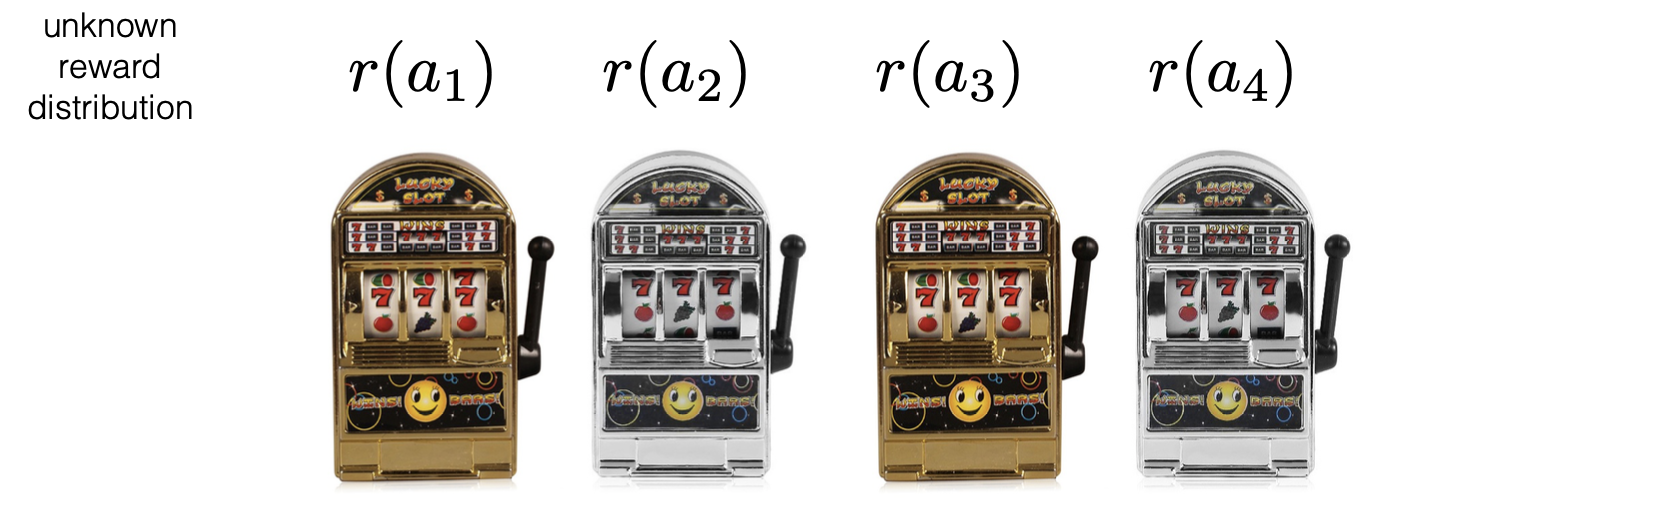
\includegraphics[width=0.8\textwidth]{figs/bandits.png}
    \caption{Multi-Armed Bandits.}
\end{figure}
In this lecture, we will introduce two algorithms: Explore-Exploit and UCB.
\begin{figure}[t]
    \centering
    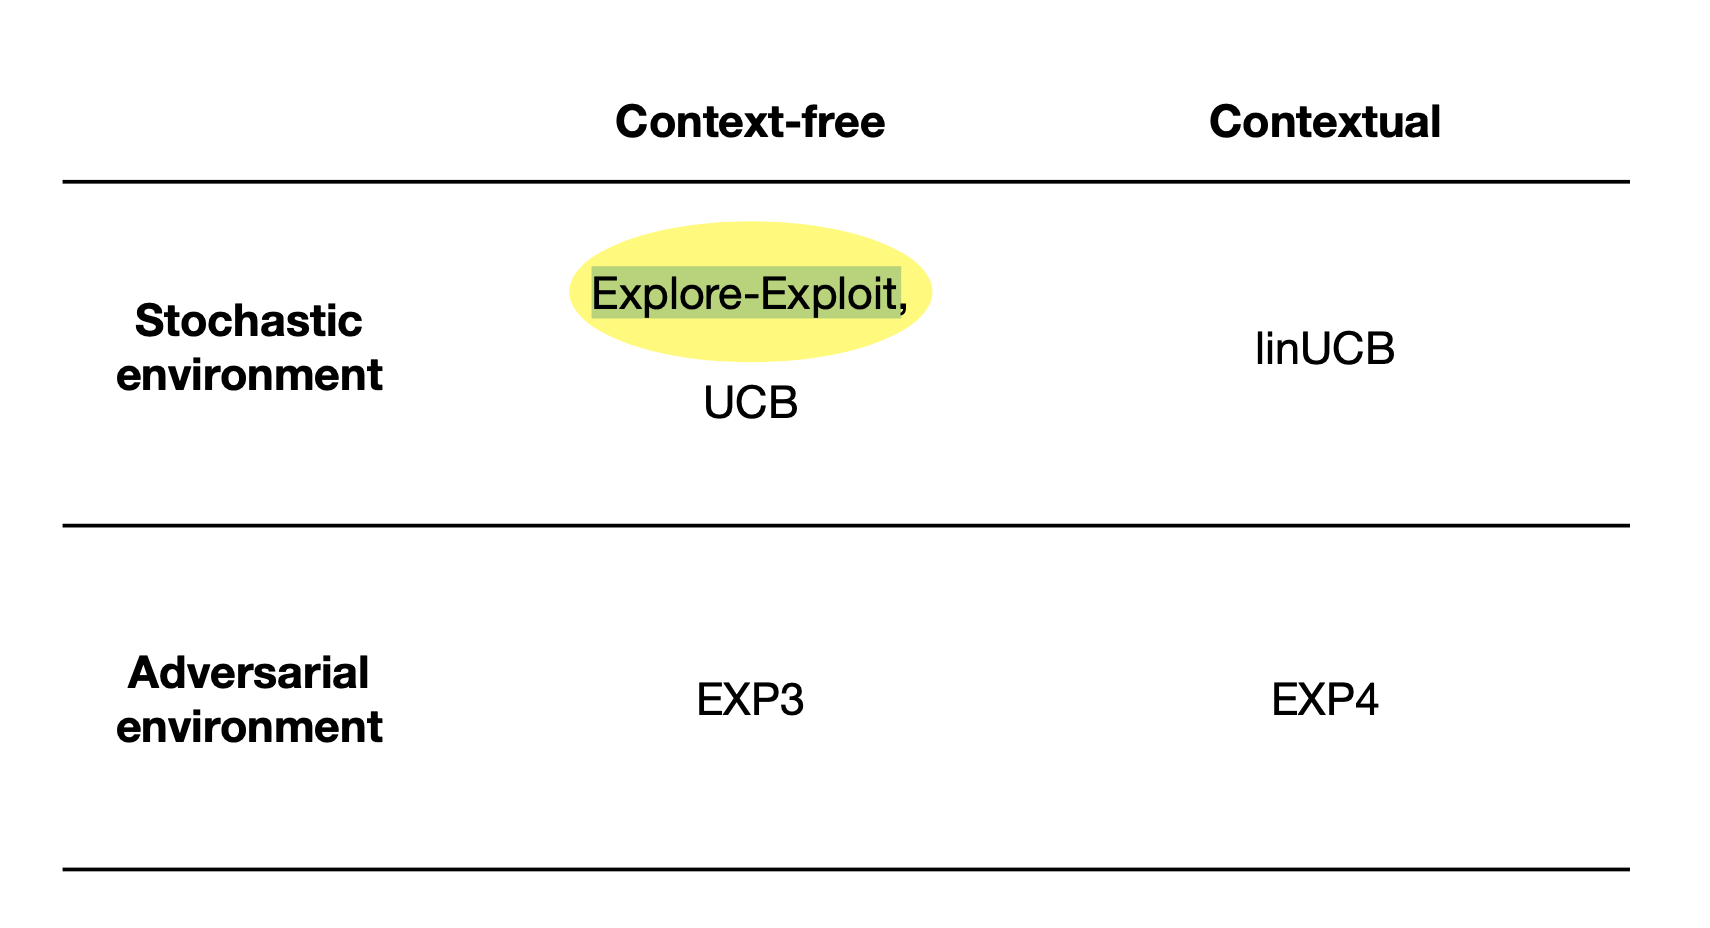
\includegraphics[width=0.6\textwidth]{figs/types.png}
    \caption{Types of MAB algorithms.}
\end{figure}

\section{Explore-Exploit}
On a very high level, the explore-exploit algorithm contains two phases:
\begin{itemize}
    \item \textbf{Explore Phase:} Pull each arm $M$ times to estimate the mean reward.
    \item \textbf{Exploit Phase:} Next keep pulling the arm with the highest expected mean reward until T.
\end{itemize}

\subsection{Notation}
Let's first introduce the notation that will be of use:
\begin{itemize}
    \item $a_k \in \mathcal{A}$: action (arm)
    \item $|\mathcal{A}| = K$: dimension of the action space
    \item $r^{(t)}$: reward (received at time t)
    \item $M$: Number of exploration steps (per action)
    \item $\widehat{\mu}_k$: Estimated average reward of action $k$
\end{itemize}

\subsection{Algorithm}
Now we provide the psuedocode of the algorithm in 
Alg.~\ref{algo:exp2}.

\begin{algorithm}[H]
\caption{Explore-Exploit}
\label{algo:exp2}
\begin{algorithmic}[1]
\REQUIRE $M$
\FOR{$k=1,\;\cdots,\;K$}
\FOR{$m=1,\;\cdots,\;M$}
\STATE $a = k$
\STATE $\text{Receive}(r)$
\STATE $\widehat{\mu}_k = \widehat{\mu}_k + \frac{r}{M}$
\ENDFOR
\ENDFOR
\FOR{$t=KM,\;\cdots,\;T$}
\STATE $a^{(t)} = \arg\max_{k}\widehat{\mu}_k'$
\ENDFOR
\end{algorithmic}
\end{algorithm}

\subsection{Regret Analysis}
The algorithm, although looks simple, actually enjoys a sub-linear regret. Before we gives the theorem and proofs of the regret bound, let's first introduce one of the most well-known concentration inequality that will be helpful for our analysis.
\begin{lemma}[Hoeffding’s Inequality~\cite{hoeffding1994probability}]
Consider a one-dimension distribution $\nu$ with expectation $mu$, where any sample $r \sim \nu$ bounded such that $r \in [0,1]$. Given $T$ i.i.d. samples $\{r^{(t)}\}_{t=1}^T$, we have that for any $\epsilon$, 
\[\mathbb{P}\left( \left|\frac{1}{T} \sum_{t=1}^T  r^{(t)}-\mu\right| \geq \epsilon \right) \leq 2\exp{(-2T\epsilon^2)}.\]
\end{lemma}

Then we can see that if the above inequalities holds, we will have 
\[\mathbb{P}\left( \left|\frac{1}{T} \sum_{t=1}^T  r^{(t)}-\mu\right| < \epsilon \right) \geq 1- 2\exp{(-2T\epsilon^2)}.\]
Now if we want the inequality to hold for some high probability, say with probability $1-\delta$ where $\delta$ is small, we can then plug in $\delta$ into the above inequality and solve for $\epsilon$:
\[\delta = 2\exp{(-2T\epsilon^2)}.\]
With some algebra we get:
\[\epsilon = \sqrt{\frac{\log(2/\delta)}{2T}}.\]
This threshold, $\epsilon$, is called ``confidence interval" or ``confidence bound", as illustrated in Fig.~\ref{fig:confid}.
\begin{figure}[t]
    \centering
    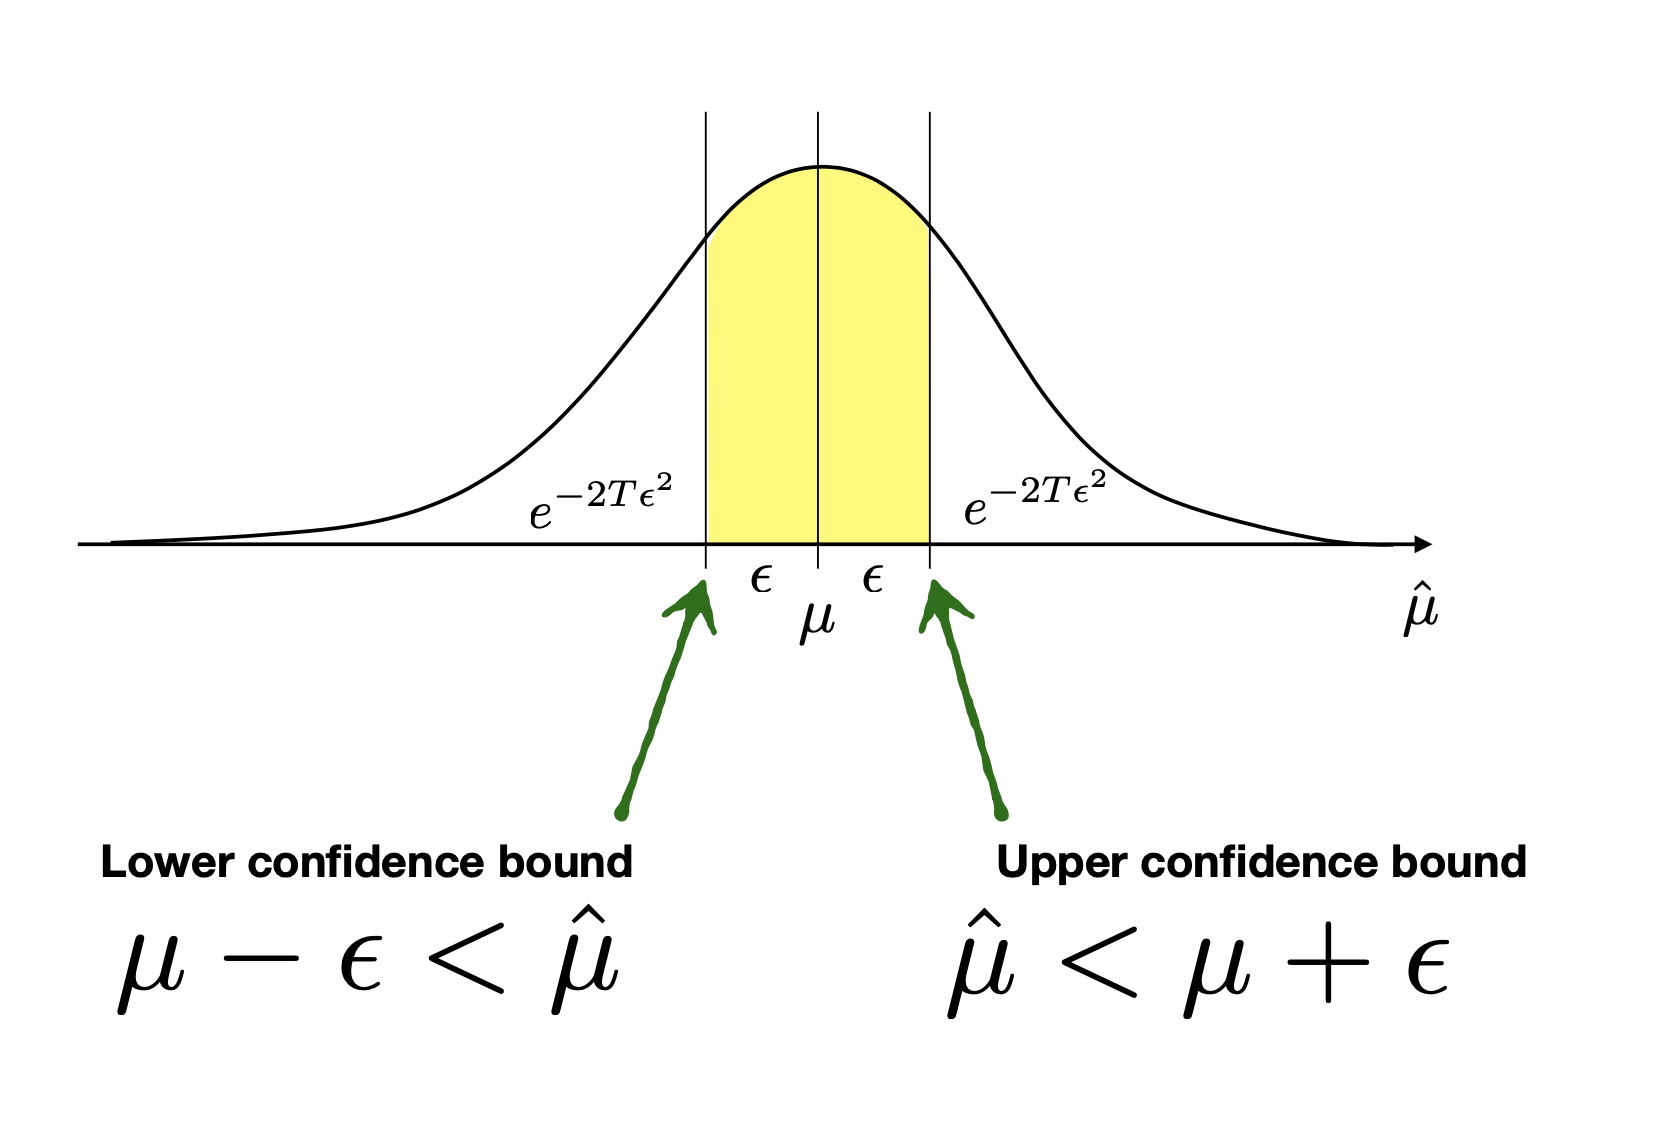
\includegraphics[width=0.5\textwidth]{figs/confidence_region.png}
    \caption{An illustration of confidence interval.}
    \label{fig:confid}
\end{figure}

Now we are ready to provide the regret bound of Explore-Exploit algorithm:
\begin{theorem}
[Regret Bound for Explore-Exploit] The regret bound of Explore-Exploit is:
\[R = \widetilde{\mathcal{O}}(K^{1/3}T^{2/3}).\]
\end{theorem}
\begin{proof}
Let's first bound the regret in the exploring phase: suppose in the worst case, each pull gives us 0 reward but the best is 1, then with $KM$ pulls in the exploring phase, we have 
\[R_{\text{explore}} = \mathcal{O}(KM).\]
In the exploitation phase, if we pulled the wrong (not the true best) arm, that means our estimate was wrong:
\[\widehat{\mu}_{\widehat{k}} \geq \widehat{\mu}_{k^{\ast}},\]
where $\widehat{k} = \arg\max_{k} \widehat{\mu}_k $ and $k^{\ast} = \arg\max_{k} \mu_k$. And this will serve as our potential function (thus we need to upper bound the LHS and lower bound the RHS and then combine). \\
To upper bound the LHS, recall that using Hoeffding we get the upper confidence bound of $\widehat{\mu}_{\widehat{k}}$:
\[\widehat{\mu}_{\widehat{k}} \leq \mu_{\widehat{k}} + \epsilon = \mu_{\widehat{k}} + \sqrt{\frac{\log(2/\delta)}{2M}}.\]
So similarly, we can lower bound the RHS by its lower confidence bound:
\[\widehat{\mu}_{k^{\ast}} \geq \mu_{k^{\ast}} = \mu_{k^{\ast}} - \sqrt{\frac{\log(2/\delta)}{2M}}.\]
Combine the above two inequalities we get:
\[\mu_{k^{\ast}} - \mu_{\widehat{k}} \leq 2\sqrt{\frac{\log(2/\delta)}{2M}}. \]
Thus we can bound the regret in the exploitation phase:
\begin{align*}
    R_{\text{exploit}} &= (T-MK)(\mu_{k^{\ast}} - \mu_{\widehat{k}})\\
    &\leq (T-MK)2\sqrt{\frac{\log(2/\delta)}{2M}}\\
    &\leq \mathcal{O}\left(2(T-MK) \sqrt{\frac{1}{M}}\right).
\end{align*}
Since the overall regret is just the sum of the regrets in the two phases, we have:
\begin{align*}
    R &= R_{\text{explore}} + R_{\text{exploit}} \\
    &\leq \mathcal{O}(MK) +  \mathcal{O}\left(2(T-MK) \sqrt{\frac{1}{M}}\right)\\
    &\leq \mathcal{O}(K^{1/3}T^{2/3}),
\end{align*}
where in the second inequality we take $M = \left(\frac{T}{K}\right)^{2/3}.$
\end{proof}
Now we can see that Explore-Exploit is a no regret algorithm!

\section{UCB}
Now we introduce the UCB algorithm. It is similar to Explore-Exploit algorithm in the sense that it also take use of the upper confidence bound, but here we skip the explore phase and directly use the upper confidence bound as a bonus at each timestep.
\subsection{Notation}
As usual, let's first introduce the notation:
\begin{itemize}
    \item $k^{(t)}$: the arm pulled at time $t$
    \item $r^{(t)}$: reward received at time $t$
    \item $T_k^{(t)}$: number of times arm $k$ was pull up to time $t$
    \item $\mu_k$: true mean reward of arm $k$
    \item $\widehat{\mu}_k^{(t)}$: estimated mean reward of arm $k$ at time $t$
    \item $T$ time horizon
\end{itemize}

\subsection{Algorithm}
Now we provide the algorithm in Alg.~\ref{algo:UCB}.

\begin{algorithm}[H]
\caption{UCB}
\label{algo:UCB}
\begin{algorithmic}[1]
\REQUIRE $\delta, T$
\FOR{$t=1,\;\cdots,\;T$}
\IF{$t \leq k$} 
\STATE $k = t$
\ELSE
\STATE $k = \arg\max_{k'} \left( \widehat{\mu}_{k'} + \sqrt{\frac{\log(2T/\delta)}{2T^{(t-1)}_{k'}}} \right)$
\ENDIF
\STATE $\text{Receive}(r^{(t)})$
\STATE $T^{t}_k = T^{(t-1)}_k + 1$
\STATE $T^{t}_{k'} = T^{(t-1)}_{k'}\; \forall k' \in [K]\setminus \{k\}$
\STATE $\widehat{\mu}_k = \frac{1}{T_{k}^{(t)}}\left( T^{(t-1)}_k \widehat{\mu}_k + r^{(t)}_k \right)$
\ENDFOR
\end{algorithmic}
\end{algorithm}

\subsection{Regret Analysis}
Before we give out the regret bound on UCB, we first introduce the following lemma:
\begin{lemma}[Union Bound]
Let $x_i$ be a set of random variables. We have
\[\mathbb{P}\left(\bigcup_i x_i\right) \leq \sum_i \mathbb{P}(x_i).\]
\end{lemma}
But how is this lemma going to help? With this lemma, now we can bound the probability of events for every round. I.e., 
\begin{align*}
    \mathbb{P}\left( \bigcup_{t=1}^{T} |\widehat{\mu}_k^{(t)} - \mu_k| > \sqrt{\frac{\log(2/\delta)}{2T^{(t)}_k}} \right) &\leq \sum_{t=1}^T \mathbb{P}\left(  |\widehat{\mu}_k^{(t)} - \mu_k| > \sqrt{\frac{\log(2/\delta)}{2T^{(t)}_k}} \right)\\
    &\leq T\delta.
\end{align*}
Then let $\delta' \triangleq T\delta$ we get 
\begin{equation}
    \epsilon' = \sqrt{\frac{\log(2T/\delta')}{2T^{(t)}_k}}.
\label{union_heoff}
\end{equation}
With these knowledge equipped, we are ready to present the regret bound for UCB algorithm:
\begin{theorem}[Regret bound for UCB]
The regret bound for UCB is:
\[R = \mathcal{O}\left( 2\sqrt{\log(2T/\delta)\sqrt{KT}} \right) = \widetilde{\mathcal{O}}(\sqrt{KT}).\]
\end{theorem}
\begin{proof}
Similar to the exploit phase in Explore-Exploit, note that if we make a mistake (pulling the non-optimal arm) in round $t$, we have:
\[\widehat{\mu}_{k} + \sqrt{\frac{\log(2T/\delta)}{2T^{(t)}_{k}}} \geq \widehat{\mu}_{k^{\ast}} + \sqrt{\frac{\log(2T/\delta)}{2T^{(t)}_{k^{\ast}}}}.\]
Again let upper bound the LHS and lower bound the RHS with what we get in Eq.~\ref{union_heoff}.\\
For the LHS:
\[\widehat{\mu}_{k} + \sqrt{\frac{\log(2T/\delta)}{2T^{(t)}_{k}}} \leq \mu_{k} + 2\sqrt{\frac{\log(2T/\delta)}{2T^{(t)}_{k}}}.\]
For the RHS:
\begin{align*}
    \widehat{\mu}_{k^{\ast}} + \sqrt{\frac{\log(2T/\delta)}{2T^{(t)}_{k^{\ast}}}} &\geq \left(\mu_{k^{\ast}} - \sqrt{\frac{\log(2T/\delta)}{2T^{(t)}_{k^{\ast}}}}\right) + \sqrt{\frac{\log(2T/\delta)}{2T^{(t)}_{k^{\ast}}}} \\
    &= \mu_{k^{\ast}} .
\end{align*}
Combine we have
\[\mu_{k} + 2\sqrt{\frac{\log(2T/\delta)}{2T^{(t)}_{k}}} \geq \mu_{k^{\ast}} .\]
Finally we have:
\begin{align*}
    R &= \sum_{t=1}^T (\mu_{k^{\ast}}- \mu_{k})\\
    & \leq \sum_{t=1}^T 2\sqrt{\frac{\log(2T/\delta)}{2T^{(t)}_{k}}} \\
    &= \frac{1}{2}\sqrt{\log(2T/\delta)} \sum_{t=1}^T \sqrt{\frac{1}{T^{(t)}_{k}}} \\
    &= \frac{1}{2}\sqrt{\log(2T/\delta)} \sum_{t=1}^T \sum_{j=1}^K \mathbbm{1}\{k^{(t)} = j\} \sqrt{\frac{1}{T^{(t)}_{j}}}\\
    &= \frac{1}{2}\sqrt{\log(2T/\delta)} \sum_{j=1}^K \sum_{t=1}^T  \mathbbm{1}\{k^{(t)} = j\} \sqrt{\frac{1}{T^{(t)}_{j}}}\\
    &= \frac{1}{2}\sqrt{\log(2T/\delta)} \sum_{j=1}^K \sum_{t=1}^{T^{(T)}_j} \sqrt{\frac{1}{t}}\\
    & \leq \sqrt{\log(2T/\delta)} \sum_{j=1}^K \sqrt{T^{(T)}_j}\\
     & \leq \sqrt{\log(2T/\delta)}  K \sqrt{\frac{1}{K}\sum_{j=1}^K T^{(T)}_j}\\
     & = \sqrt{\log(2T/\delta)}  K \sqrt{\frac{T}{K}}\\
     &= \sqrt{\log(2T/\delta)}  \sqrt{KT}\\
     &= \widetilde{\mathcal{O}}(\sqrt{KT}).
\end{align*}
Here the second inequality is by $\sum_{t=1}^T \sqrt{\frac{1}{t}} \leq 2\sqrt{T}$ and the third inequality is Jensen's inequality.
\end{proof}
\newpage
{
\bibliography{lec12refs}
\bibliographystyle{abbrv}
}

%\section{Appendix}
%This section provides any relevant background material that was not covered in the lectures, but was found to be useful for understanding the material. 
%For example, derivations, theory underlying techniques employed, etc. 

%Additionally, this section can summarizes applications or extensions of these techniques found in the literature. 

\end{document} % Done!


